\documentclass[a4paper, fleqn]{article}

\usepackage{amsmath}
\usepackage{enumitem}
\usepackage{graphicx}

\begin{document}

\title{Lab Exercise II \\ Making Maps I: Introduction to Spatial Analysis, Data Visualization and Map Design}
\author{Basil R. Yap}
\date{2018 February 01}
\maketitle

\section{Part I}

\begin{itemize}
\item \textbf{Figure 1}: 50936 meters\\
In the vector layer, a new calculated field was added using in-built function "\$length".\\
\begin{figure}[h!]
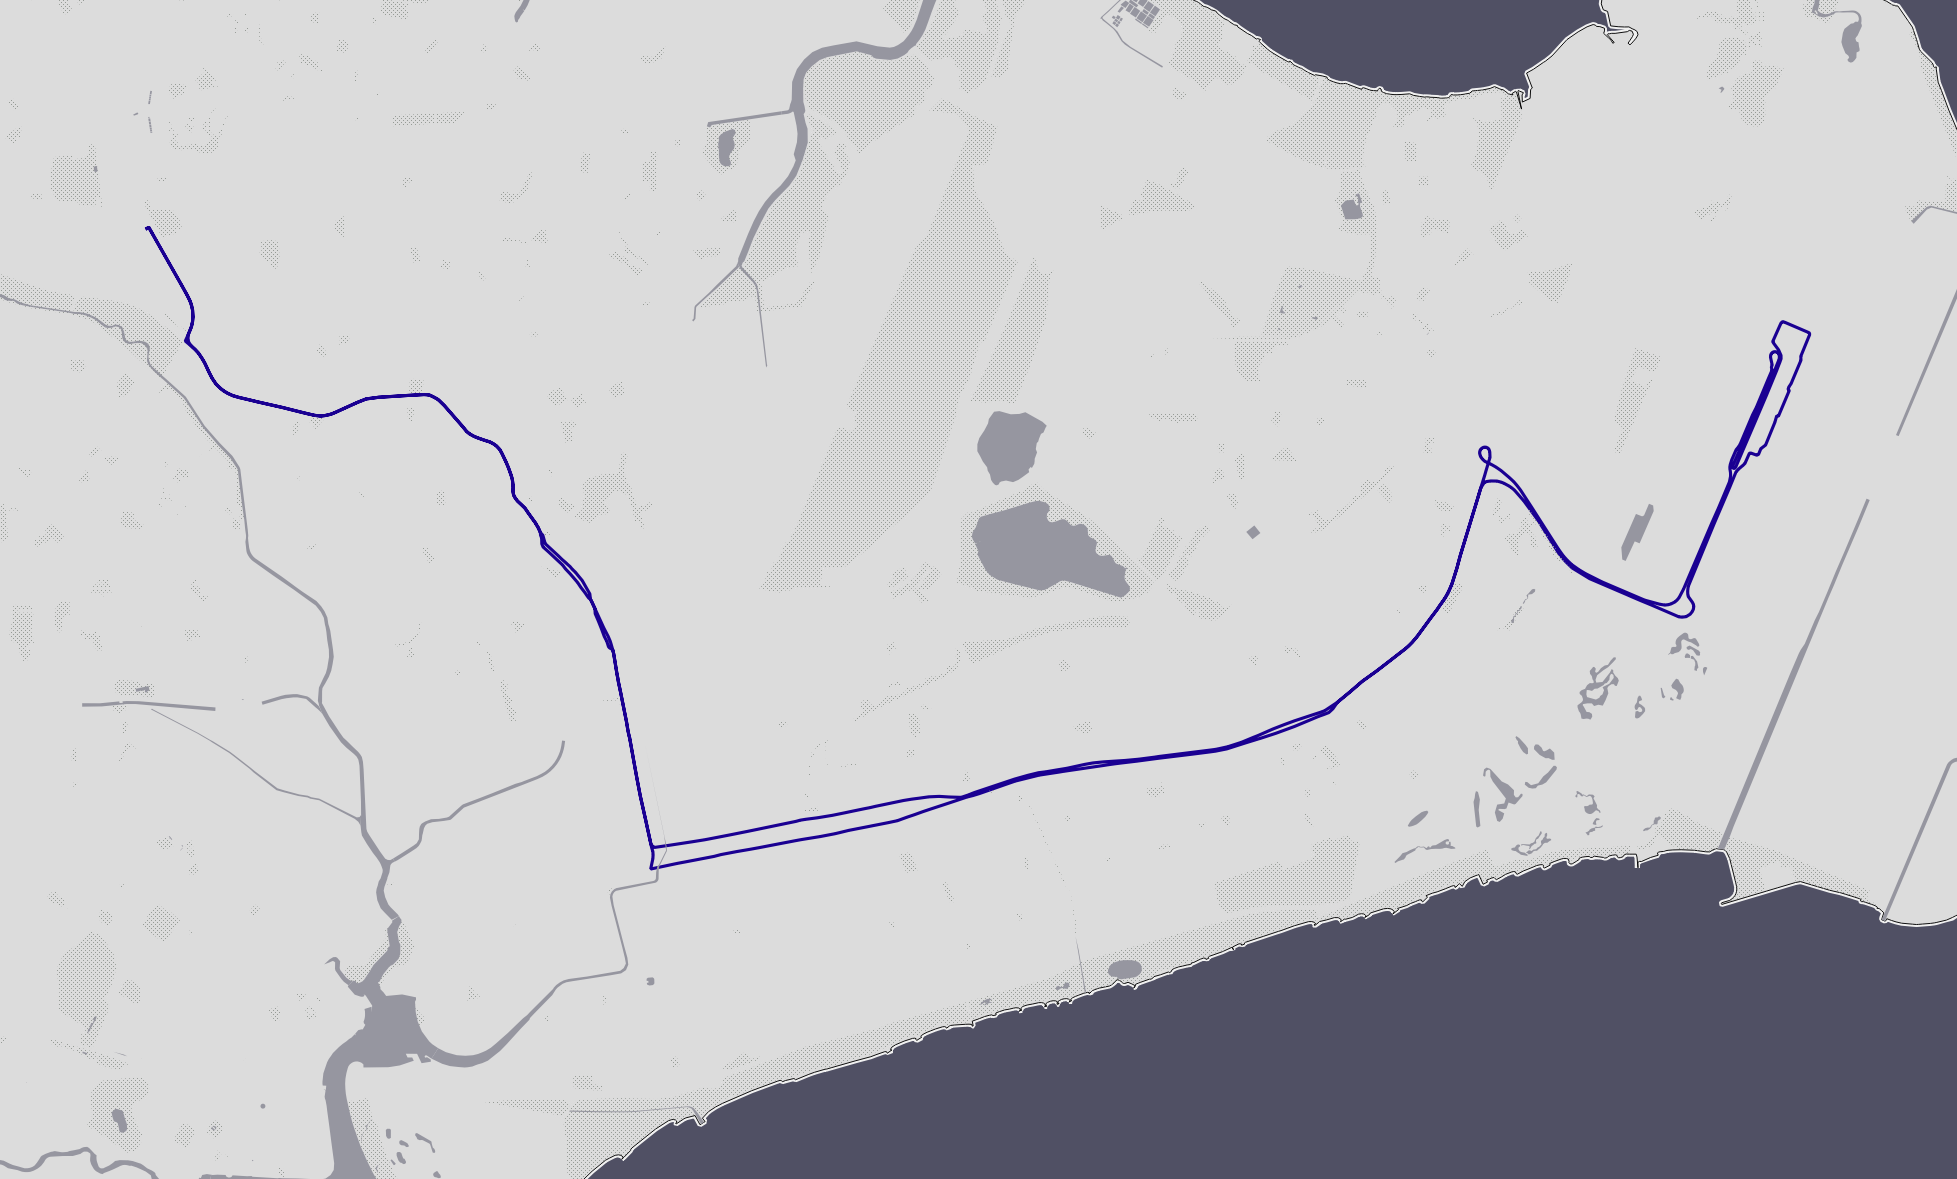
\includegraphics[width=\linewidth]{./assets/201802071736.png}
\caption{Length of Line 24}
\label{figure:map1}
\end{figure}
\pagebreak
\item \textbf{Figure 2}: You could visualize the data using a higher granularity to show concentration at smaller scale.\\
\begin{figure}[h!]
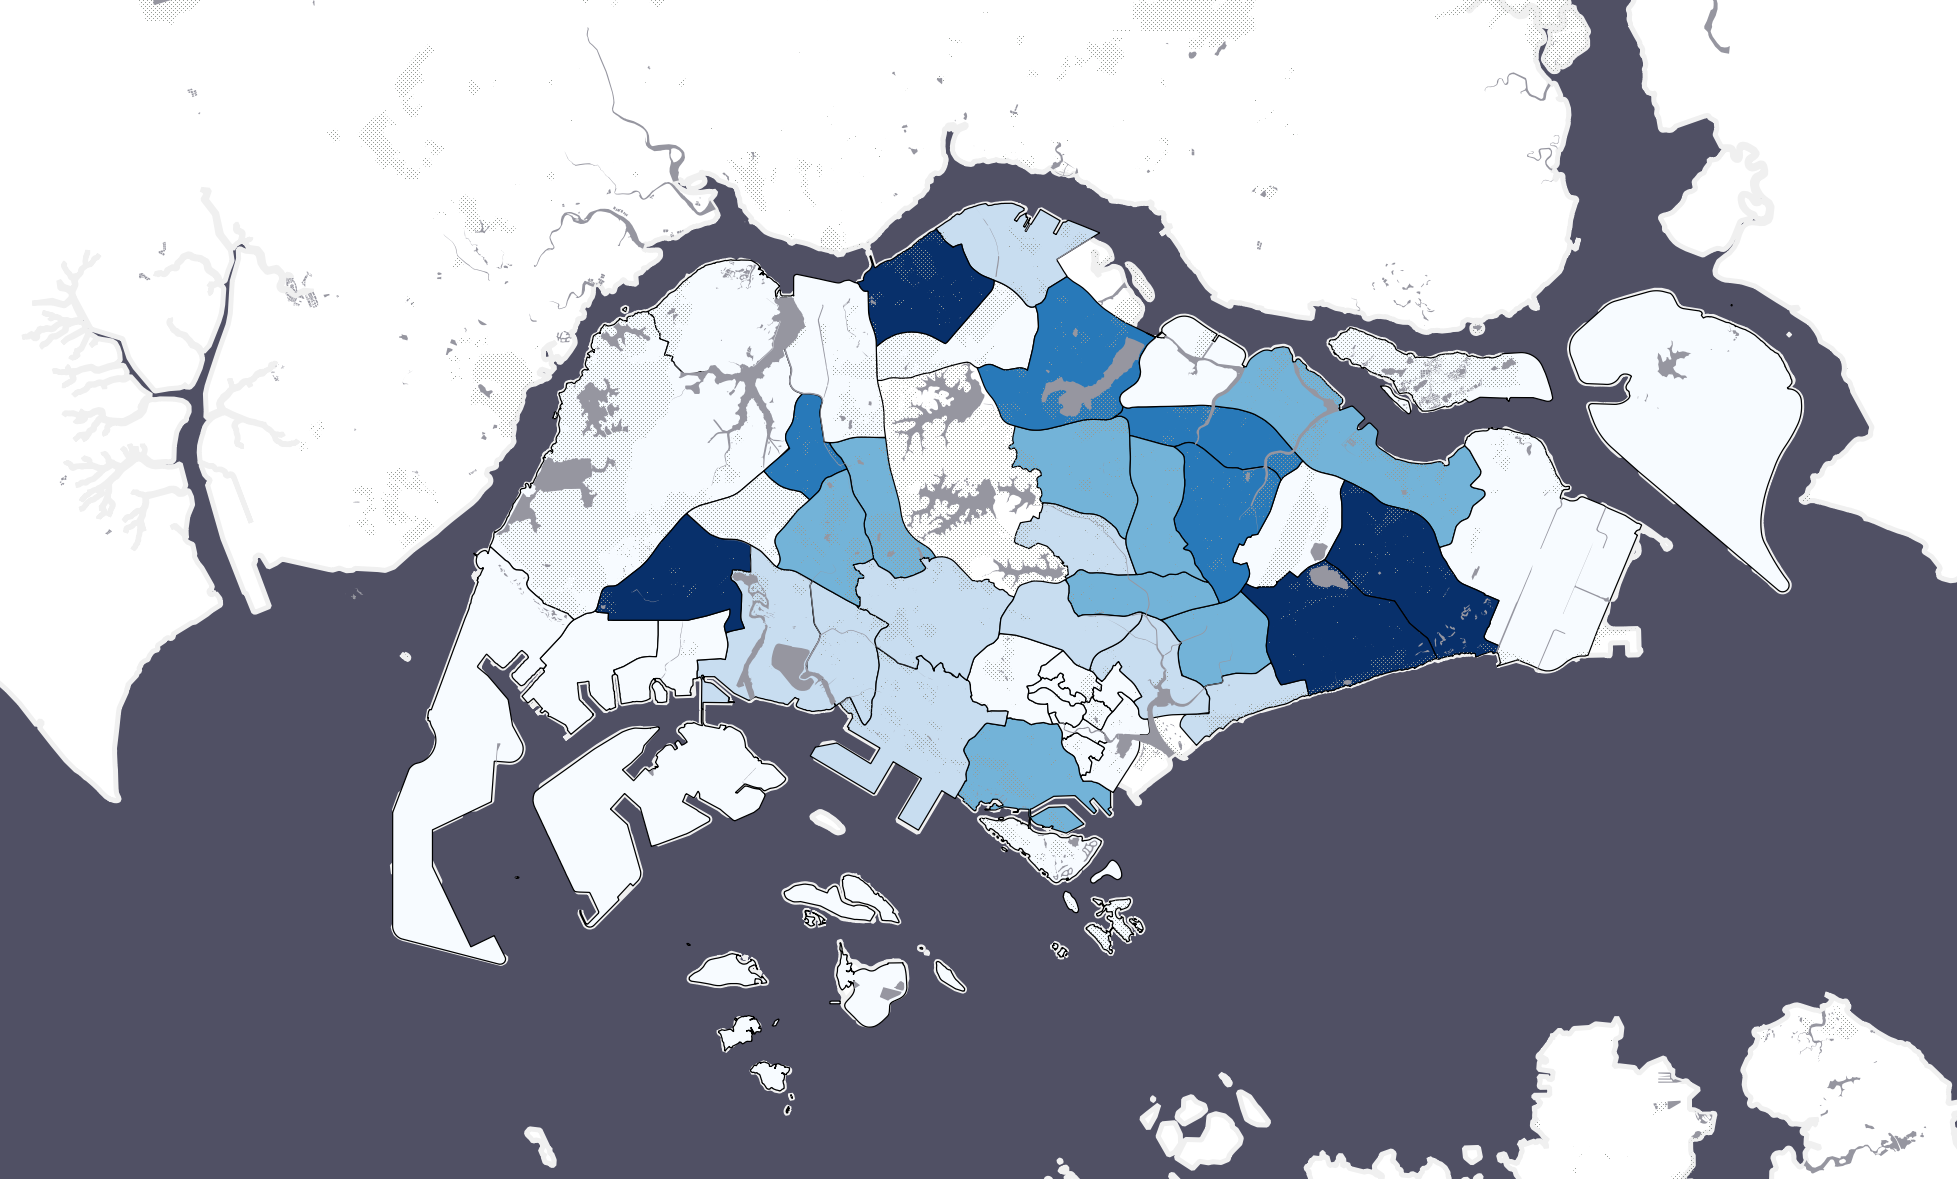
\includegraphics[width=\linewidth]{./assets/201802071800.png}
\caption{Concentration of Population in Singapore}
\label{figure:map2}
\end{figure}
\end{itemize}
\pagebreak
\section{Part II}

\subsection{Question 1}

\begin{enumerate}[label=(\alph{*})]
\item \textbf{Figure 3}\\
\begin{figure}[h!]
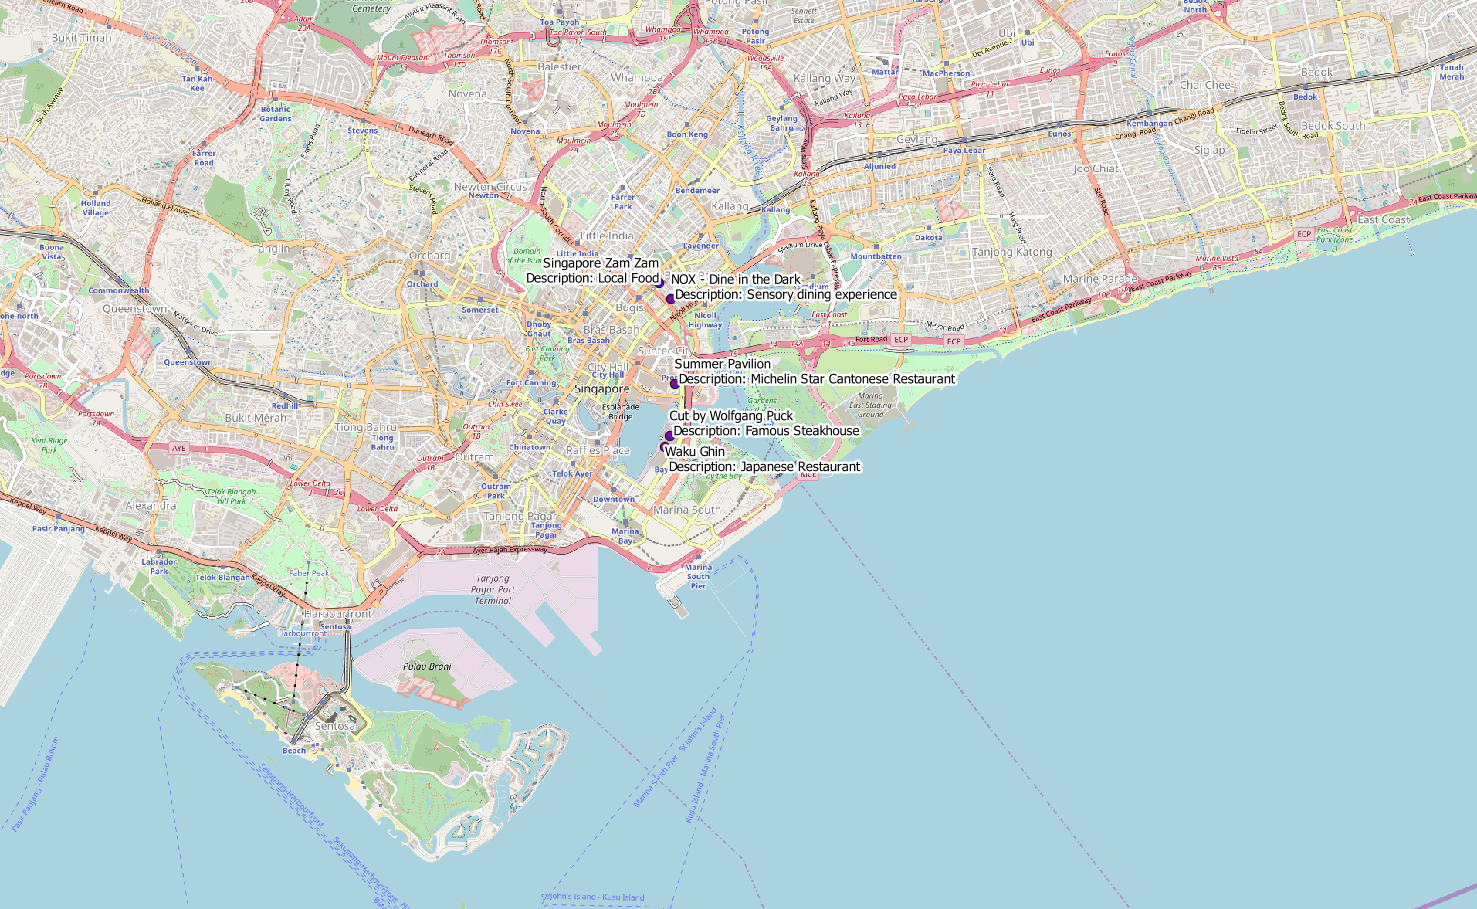
\includegraphics[width=\linewidth]{./assets/201802071629.png}
\caption{Top 5 Restaurants in Singapore (with Labels)}
\label{figure:map3}
\end{figure}

\pagebreak

\item \textbf{Figure 4}\\
\begin{figure}[h!]
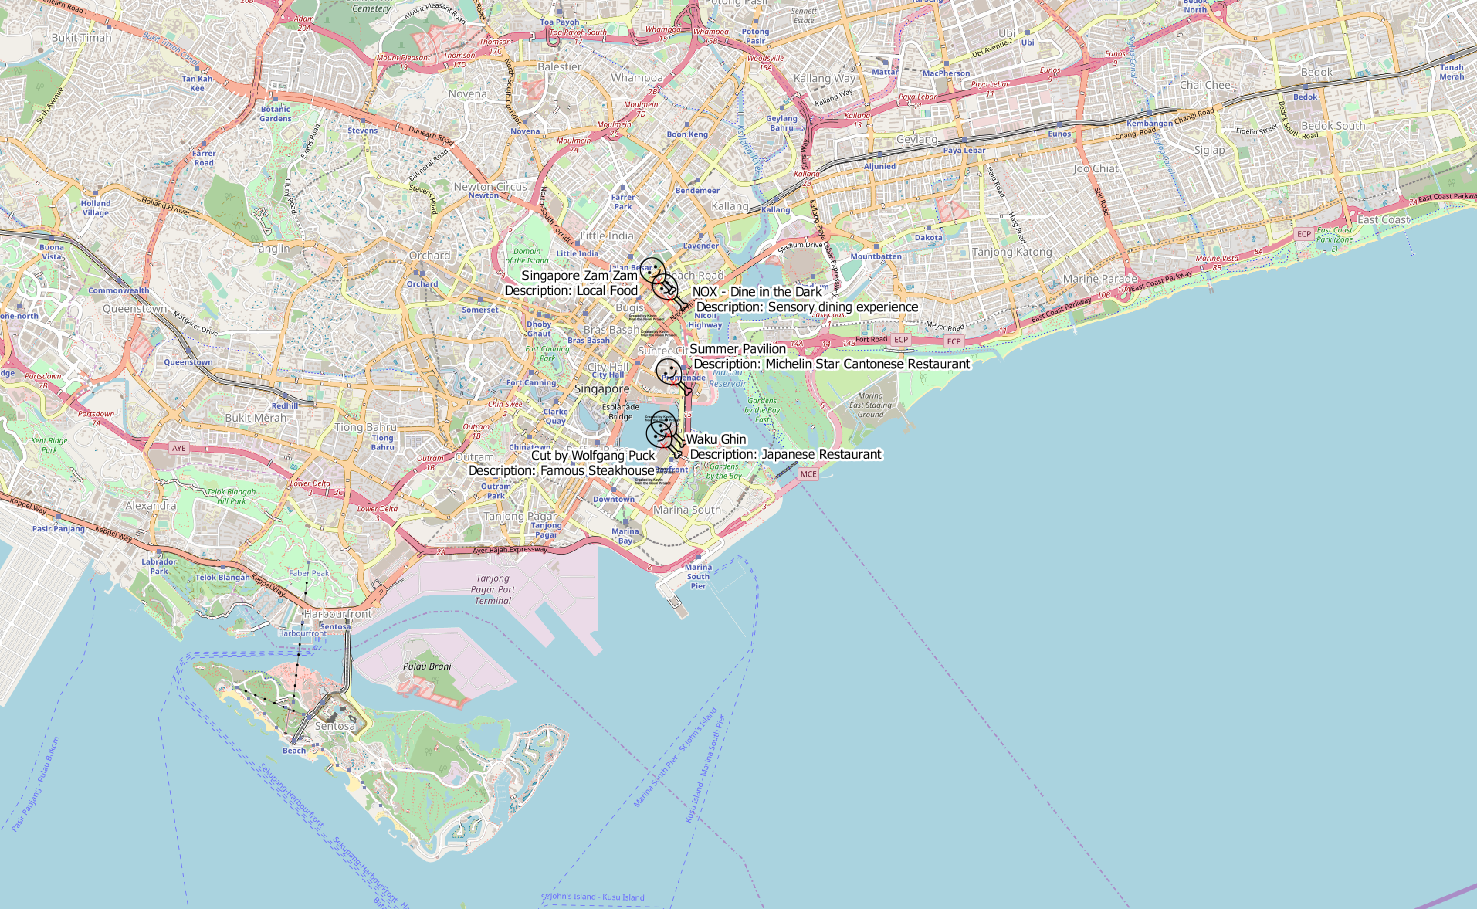
\includegraphics[width=\linewidth]{./assets/201802071645.png}
\caption{Top 5 Restaurants in Singapore (with Icons)}
\label{figure:map4}
\end{figure}
\end{enumerate}

\subsection{Question 2}

\begin{enumerate}[label=(\alph{*})]
\item \textbf{Figure 5}\\
\begin{figure}[h!]
\begin{center}
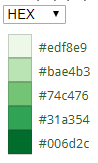
\includegraphics{./assets/201802071807.png}
\caption{Sequential Color Scale}
\label{figure:image1}
\end{center}
\end{figure}
\pagebreak
\item \textbf{Figure 6}\\
\begin{figure}[h!]
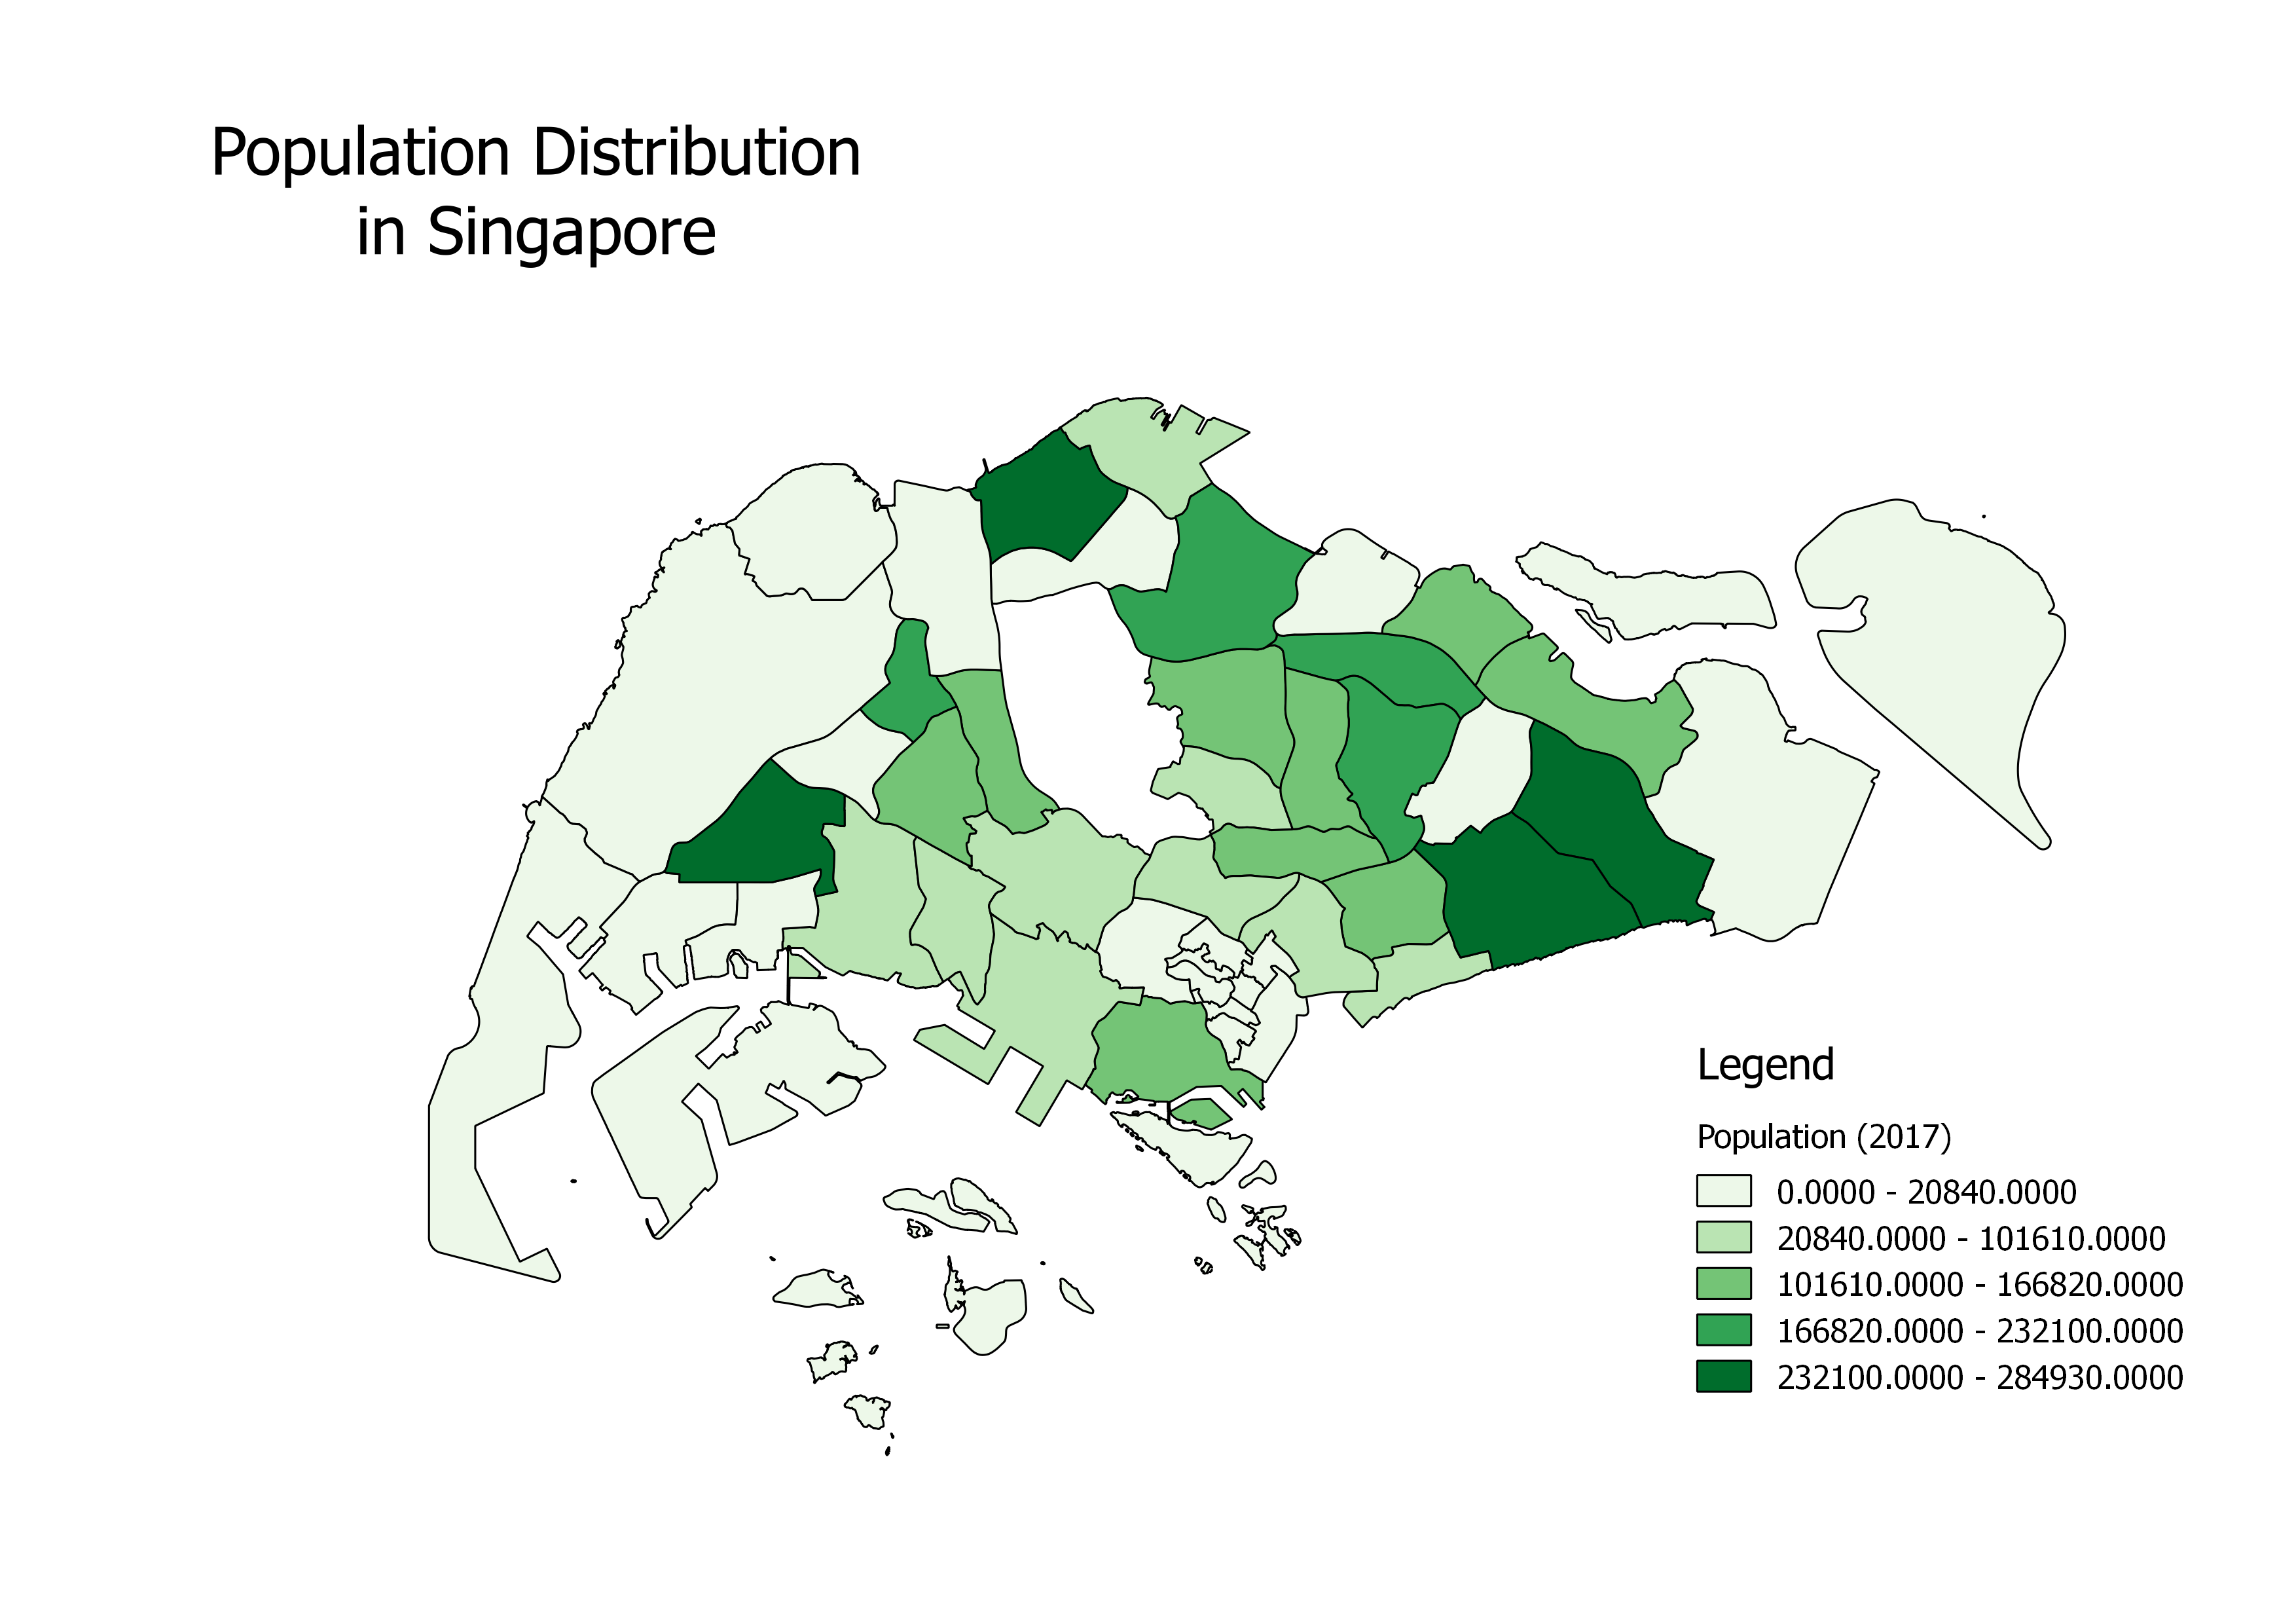
\includegraphics[width=\linewidth]{./assets/201802071823.png}
\caption{Population Distribution in Singapore (2017)}
\label{figure:map5}
\end{figure}
\end{enumerate}

\end{document}